\subsection{Centrality}
Following from identifying communities within a social network, it is also apparent that establishing the most \emph{central} or \emph{important} person is within a community. This person is most likely going to have a large influence over the members of the community.

\subsubsection{Degree Centrality}
The degree centrality is a simple measure to produce for a social network. For an undirected graph (relationships are symmetric), the degree centrality for a vertex, \emph{v}, is simply the number of edges connected to it. For a directed graph, say the network of Twitter\footnote{\url{http://twitter.com/}} users following, and being followed by others, two measures are defined, the in-degree and out-degree. These are simply the number of incoming and outgoing edges respectively.

Whilst a fairly simple measure to compute, degree centrality can be useful. A person with a high degree centrality is likely to hold a larger influence amongst the people they share a connection with, as they are more popular. \cite[p.~169]{newman10} suggests that the number of citations an academic paper receives can be used as its in-degree centrality, and is a crude measure of whether the paper was influential and as such had an impact on scientific research.

\subsubsection{Eigenvector Centrality}
The eigenvector centrality measure identifies important vertices within a graph by awarding each vertex a score proportional to the to the sum of the centralities of adjacent vertices. This means that a vertex has a high centrality because it either has many neighbours, or because its neighbours have a high centrality themselves \cite{newman10}.

\subsubsection{PageRank}
The PageRank algorithm \cite{pagerank} developed by Google is a further extension of the eigenvector centrality measure. The centrality score awarded to each vertex is proportional to the centrality of its neighbours divided by the number of outgoing connections. The PageRank algorithm was devised to rank webpages based on the quality and quantity of the incoming links to that webpage.

A simplified version of PageRank can be defined as, where $u$ is the vertex to be ranked, $B_u$ is the set of vertices with edges incident on $u$, $N_v$ is the number of outgoing edges from $v$, and $c$ is a factor used for normalisation \cite{pagerank}:

\begin{equation}
R(u) = c \sum_{v \in B_u} \frac{R(v)}{N_v}
\label{eq:simplepagerank}
\end{equation}

Equation \ref{eq:simplepagerank} does not take into account of two properties which can exist within a directed graph, rank sinks and dangling links. A rank sink is a closed loop within the graph, which has incoming edges, but no edges leaving the loop. As such, these loops 'keep' the PageRank which enters them and can artificially cause these vertices to be ranked higher. A dangling link is similar, but is just a vertex with no outgoing edges. The approach taken by \citeauthor{pagerank} is to remove any of these dangling links from the graph, and if this produces new dangling links, remove these new dangling links and repeat until no dangling links remain.

\begin{figure}
  \centering
  \subfloat[A simple rank sink]{\label{fig:ranksink}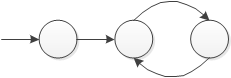
\includegraphics[width=0.4\textwidth]{./img/ranksink}}
  ~ 
  \subfloat[A dangling link]{\label{fig:danglinglink}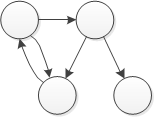
\includegraphics[width=0.3\textwidth]{./img/danglinglink}}
  ~ 
  
  \caption{Problems with simplified PageRank}
  \label{fig:pagerank}
\end{figure}

This simplified PageRank makes use of the \emph{random surfer model}, which simulates that for each outgoing link from a webpage, a user randomly selects on of these links, and continues browsing. A real user would not continue in this fashion if the outgoing links from successive webpages form a loop, they would navigate to a new webpage not linked by these pages, based on the distribution factor $E$. This is modelled within PageRank as a rank source:

\begin{equation}
R'(u) = c \sum_{v \in B_u} \frac{R'(v)}{N_v} + cE(u)
\label{eq:pagerank}
\end{equation}

The rank source is the amount of rank each vertex in the graph contributes to the system. This models the behaviour of a real user and ensures that rank sinks do not accumulate rank.

\subsubsection{Closeness Centrality}
Closeness centrality is a measure of the average distance from a vertex to other vertices. A geodesic path between two vertices is the minimum number of edges required to connect them within a graph. The closeness centrality defined in equation \ref{eq:closenesscentrality1} is the sum of the length of all geodesic paths, $d_{ij}$, from a vertex, $i$, to all other vertices, $j$:

\begin{equation}
l_i = \frac{1}{n}\sum_{j} d_{ij}
\label{eq:closenesscentrality1}
\end{equation}

A slight alternative is to exclude the geodesic path $d_{ij}$ when $i = j$ because this is trivially 0, and a vertex's influence on itself is not relevant to the calculation of centrality:

\begin{equation}
l_i = \frac{1}{n-1}\sum_{j(\neq i)} d_{ij}
\label{eq:closenesscentrality2}
\end{equation}

Closeness centrality defined in equations \ref{eq:closenesscentrality1} and \ref{eq:closenesscentrality2} produce results differently to other measures of centrality, whereby a lower value for $l_i$ indicates that vertex $i$ is more central within the network. Because of this, closeness centrality can also be defined as:

\begin{equation}
C_i = \frac{1}{l_i} = \frac{n}{\sum_{j(\neq i)} d_{ij}}
\label{eq:closenesscentrality3}
\end{equation}

Equation \ref{eq:closenesscentrality3} produces results more consistent with other measures of centrality as a higher value of $C_i$ indicates vertex $i$ is more central. This equation is simply the inverse of equation \ref{eq:closenesscentrality1}.

Within a social network, a person with a high closeness centrality, defined by equation \ref{eq:closenesscentrality3}, could find that their opinions reach others in the community faster than someone with a lower closeness centrality \cite{newman10}.

\subsubsection{Betweeness Centrality}
Betweeness centrality is different measure of calculating centrality. Instead of being concerned with the quantity, or quality, of links, betweeness centrality measures the extent to which a vertex lies on paths between other vertices.

\begin{figure}%
\centering
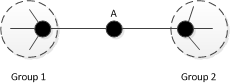
\includegraphics[width=0.4\columnwidth]{./img/betweenesscentrality}%
\caption{A low degree vertex with high betweeness \cite{newman10}}%
\label{fig:betweenesscentrality}%
\end{figure}

Betweeness centrality for a vertex $i$ is mathematically defined as the sum of the number of shortest paths, $n_{st}^{i}$, from vertex $s$ to vertex $t$ which pass through $i$, divided by the total number of shortest paths from $s$ to $t$:

\begin{equation}
x_i = \sum_{st} \frac{n_{st}^{i}}{g_{st}}
\label{eq:betweenesscentrality}
\end{equation}

Figure \ref{fig:betweenesscentrality} shows a sketch of a network which contains two distinct groups connected to each other via vertex A. All paths between the two groups must pass through vertex A, so it has a high betweeness even though its degree is low \cite{newman10}. With this example as well, it is quite likely that vertex A would score poorly with other measures of centrality, however due it forming the bridge between the two groups, vertex A is quite likely to be quite influential in controlling the flow of information between the two groups.